\section{Sammenligning af korrelerede parametre}
\label{DatabehandlingSammenligningKorrelerede}
%
Som beskrevet udføres der en PCA analyse relativt til forskellige grupperinger. Ud fra disse PCA analyser forefindes der korrelation mellem nogen af de fundne og testede parametre. For yderliger at undersøge disse korrelationer opsættes relevante grafer, hvor forholdet mellem de forskellige parametre og skala spørgsmål visualiseres. På alle grafer i det følgende afsnit vil x-aksen indikere testpersoner, men ikke nødvendigvis i kronologisk rækkefølge, hvorfor værdier på x-aksen er fjernet. Dertil er manglende besvarelser ekskluderet fra graferne, hvorfor antallet af testpersonerne varierer. Selvom dette afsnit er inddelt i tre underafsnit for henholdvis: Højde, afstand og indgangsvinkel, hvori korrelationerne fra den foregående PCA præsenteres, så bygger graferne på det samlede datasæt og tager derfor ikke højde for hverken højde, afstand eller indgangsvinkel.  

\subsection{Korrelerede parametre fra højde}
\label{DatabehandlingSammenligningKorreleredeHoejde}
%
Når PCA analysen udføres relativt til højde, tyder det, som beskrevet i \fullref{DatabehandlingRHeight}, på, at en positiv korrelation mellem følgende parametre forekommer:
%
\begin{itemize}
	\item SQ12 og SQ18
	\item SQ10 OG SQ13 
	\item SQ14 og SQ15
	\item SQ8 og SQ17\blankline
\end{itemize}
\noindent
%
Derudover forefindes der negativ korrelation mellem følgende parametre:
%
\begin{itemize}
	\item SQ12 og S21
	\item SQ18 og SQ21
	\item SQ2 og SQ9
	\item SQ4 og SQ9
	\item SQ16 og SQ19\blankline
\end{itemize}
\noindent
%
Korrelationen mellem SQ12 og SQ18 skyldes formentlig ikke, at de måler det samme men derimod, at når testpersonerne godt kan lide at blive betjent af robotten, så synes de også robotten er spændende, hvilket fremgår på \autoref{fig:SammenligningSQ12SQ18}. 
%
\begin{figure}[H]
	\centering
	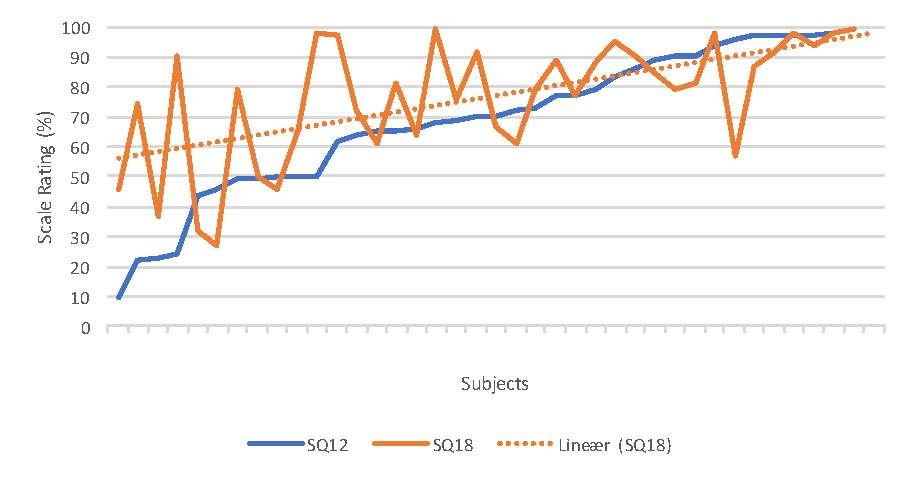
\includegraphics[width=\textwidth]{Figure/Korrelationsgrafer/SQ12+SQ18}
	\caption{Sammenhæng mellem hvad testpersonerne angiver (\%) på skalaen til SQ12: \textit{Jeg kan godt lide at blive betjent af robotten} og SQ18: \textit{Hvad synes du om robotten?}. Denne graf bygger på 38 besvarelser, da der manglede fem.}
	\label{fig:SammenligningSQ12SQ18}
\end{figure}
\noindent
%
Sammenholdes SQ10 med SQ13 forekommer der ud fra \autoref{fig:SammenligningSQ10SQ13}, tiltrods for stor variation i besvarelserne til SQ13, en positiv korrelation. Dette indikerer derfor, at når testpersonerne regnede med at robotten fulgte dem hen til det valgte sted, så var de også mere trygge ved robotten. 
%
\begin{figure}[H]
	\centering
	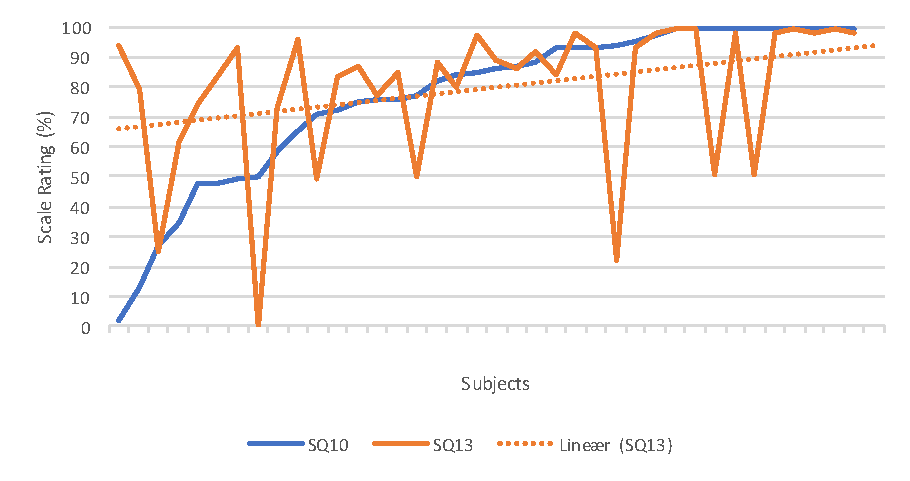
\includegraphics[width=\textwidth]{Figure/Korrelationsgrafer/SQ10+SQ13}
	\caption{Sammenhæng mellem hvad testpersonerne angiver (\%) på skalaen til SQ10: \textit{Jeg føler mig tryg ved robotten} og SQ13: \textit{Jeg regnede med, at robotten fulgte mig hen til det sted jeg valgte}. Denne graf bygger på 38 besvarelser, da der manglede fem.}
	\label{fig:SammenligningSQ10SQ13}
\end{figure}
\noindent
%
Korrelationen mellem SQ14 og SQ15 skyldes formentlig ikke, at de måler det samme, og ud fra tendenslinjen på \autoref{fig:SammenligningSQ14SQ15} tyder det på, at der tilnærmelsesvis er en sammenhæng mellem de to parametre. Fokuseres der derimod på punkterne på graferne virker det ikke som om, at der er en korrelation mellem hvor overrasket testpersonerne bliver og hvor personlig robottens hjælp opleves.
%
\begin{figure}[H]
	\centering
	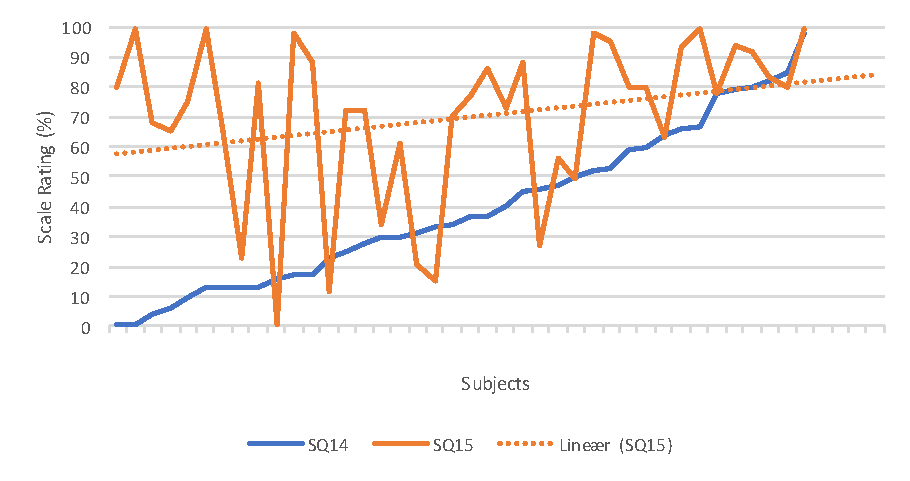
\includegraphics[width=\textwidth]{Figure/Korrelationsgrafer/SQ14+SQ15}
	\caption{Sammenhæng mellem hvad testpersonerne angiver (\%) på skalaen til SQ14: \textit{Hvor personlig oplevede du robottens hjælp?} og SQ15: \textit{Hvor overrasket blev du over robottens henvendelse?}. Denne graf bygger på 40 besvarelser, da der manglede tre.}
	\label{fig:SammenligningSQ14SQ15}
\end{figure}
\noindent
%
Korrelationen mellem SQ8 og SQ17 skyldes formentlig ikke, at de måler det sammen, det tyder derimod på, at korrelationen forekommer når testpersonerne føler, at robotten kan hjælpe dem og samtidig vurderer at robotten er elegant. Dog er denne korrelation lille, fordi datapunkterne varierer en del, særligt i forhold til SQ17, jævnfør \autoref{fig:SammenligningSQ8SQ17}.  
%
\begin{figure}[H]
	\centering
	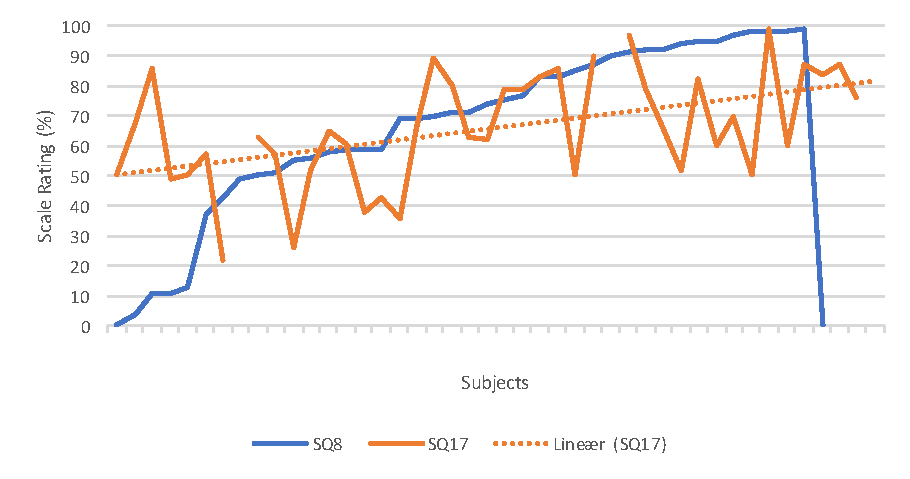
\includegraphics[width=\textwidth]{Figure/Korrelationsgrafer/SQ8+SQ17}
	\caption{Sammenhæng mellem hvad testpersonerne angiver (\%) på skalaen til SQ8: \textit{Jeg føler, at robotten kan hjælpe mig} og SQ17: \textit{Hvad synes du om robotten?}. Denne graf bygger på 38 besvarelser, da der manglede fem.}
	\label{fig:SammenligningSQ8SQ17}
\end{figure}
\noindent
I forhold til den negative korrelation mellem SQ21 og SQ12, vedrørende hvor godt testpersonerne kan lide at blive betjent af robotten, fremgår det ud fra \autoref{fig:SammenligningSQ12SQ21}, at desto mindre anmassende robotten opleves, desto bedre kan testpersonerne lide at blive betjent af robotten, hvilket giver god mening. 
%
\begin{figure}[H]
	\centering
	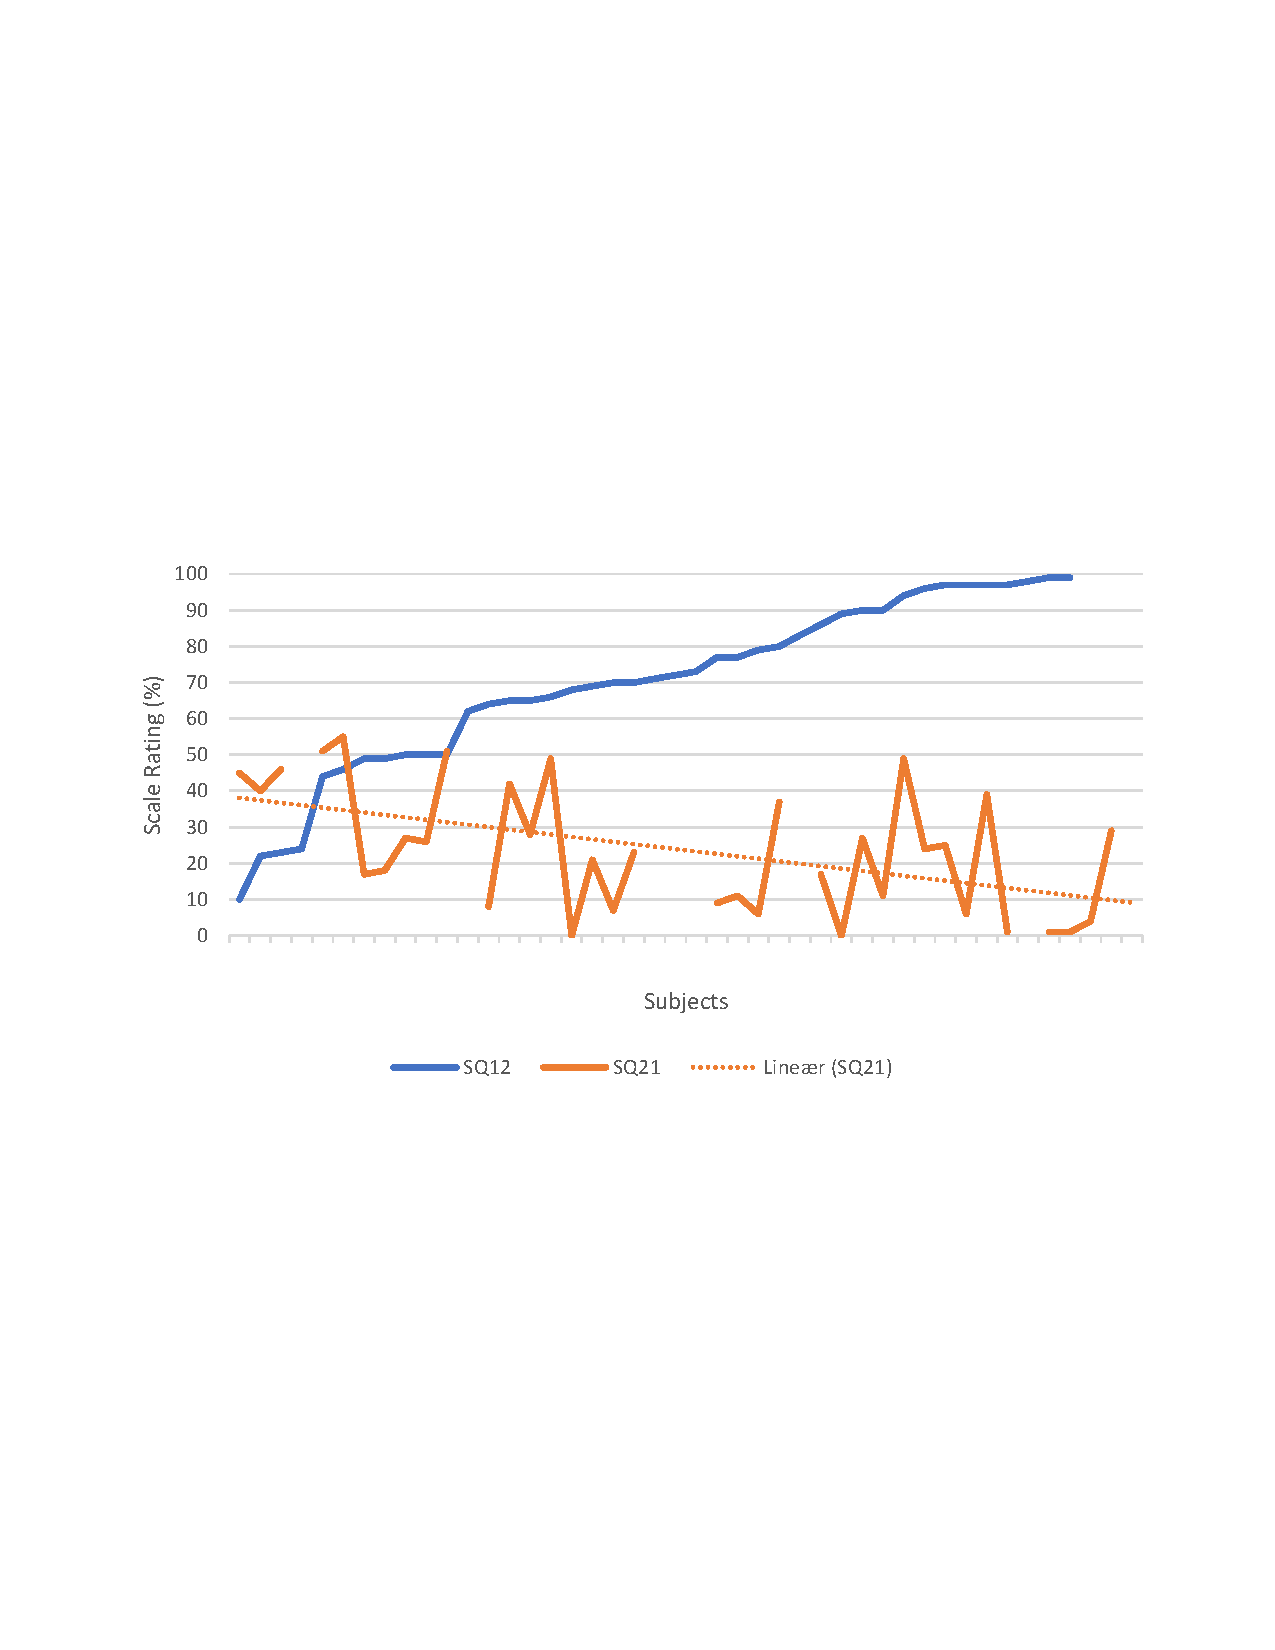
\includegraphics[width=\textwidth]{Figure/Korrelationsgrafer/SQ12+SQ21}
	\caption{Sammenhæng mellem hvad testpersonerne angiver (\%) på skalaen til SQ12: \textit{Jeg kan godt lide at blive betjent af robotten} og SQ21: \textit{Hvad synes du ellers om robotten?}. Denne graf bygger på 38 besvarelser, da der manglede fem.}
	\label{fig:SammenligningSQ12SQ21}
\end{figure}
\noindent
%
I forhold til den negative korrelation mellem SQ18, vedrørende hvor spændende robotten opleves, og SQ21 fremgår det ud fra \autoref{fig:SammenligningSQ18SQ21}, at desto mindre anmassende robotten opleves desto mere spændende vurderes robotten. Dog tyder det på, når SQ18 vurderes højest så stiger vurderingen på SQ21 ligeledes. 
%
\begin{figure}[H]
	\centering
	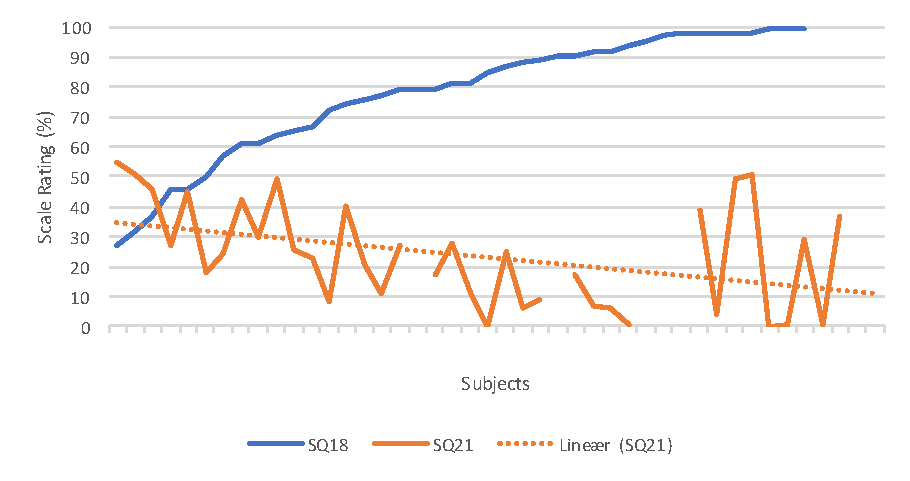
\includegraphics[width=\textwidth]{Figure/Korrelationsgrafer/SQ18+SQ21}
	\caption{Sammenhæng mellem hvad testpersonerne angiver (\%) på skalaen til SQ18: \textit{Hvad synes du om robotten?}, i forhold til \textit{spændende}, og SQ21: \textit{Hvad synes du ellers om robotten?}, i forhold til \textit{anmassende}. Denne graf bygger på 35 besvarelser, da der manglede otte.}
	\label{fig:SammenligningSQ18SQ21}
\end{figure}
\noindent
%
I henhold til den negative korrelation mellem SQ2, vedrørende hvorvidt robotten er imødekommende eller afvisende, og SQ9 fremgår det, at desto mere imødekommende robotten opleves, desto mindre er den i vejen, jævnfør \autoref{fig:SammenligningSQ2SQ9}.
%
\begin{figure}[H]
	\centering
	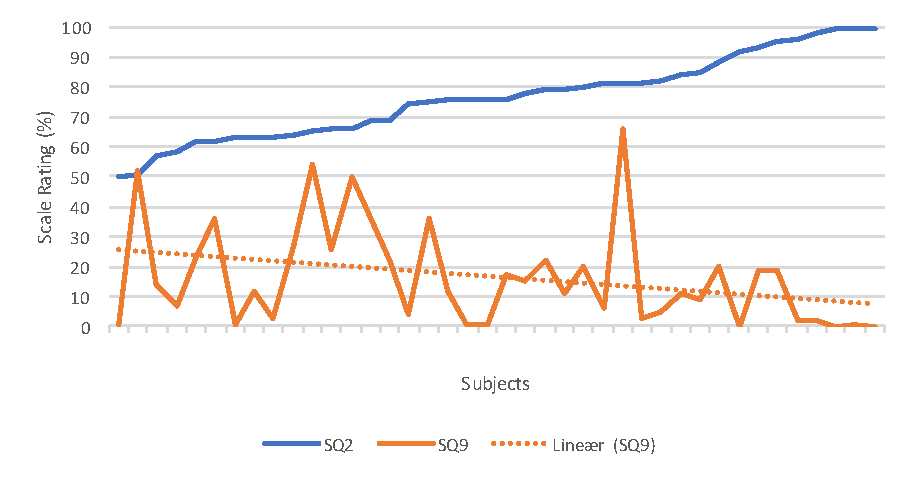
\includegraphics[width=\textwidth]{Figure/Korrelationsgrafer/SQ2+SQ9}
	\caption{Sammenhæng mellem hvad testpersonerne angiver (\%) på skalaen til SQ2: \textit{Hvordan oplevede du robotten?}, i forhold til \textit{afvisende} og \textit{imødekommende}, og SQ9: \textit{Jeg synes, at robotten stod i vejen}. Denne graf bygger på 40 besvarelser, da der manglede tre.}
	\label{fig:SammenligningSQ2SQ9}
\end{figure}
\noindent
%
Selvom det på \autoref{fig:RHeight-Biplot} tyder på, at der er en negativ korrelation mellem SQ4, vedrørende robottens bevægelser, og SQ9 så fremgår denne korrelation ikke som værende negativ på \autoref{fig:RHeight-3D} eller på \autoref{fig:SammenligningSQ4SQ9}. På \autoref{fig:SammenligningSQ4SQ9} tyder det nærmere på, at der er en svag positiv korrelation. 
%
\begin{figure}[H]
	\centering
	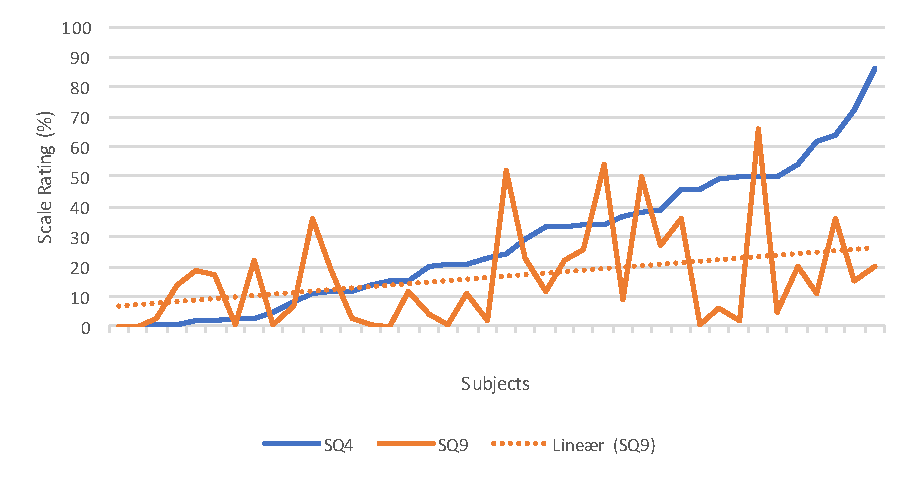
\includegraphics[width=\textwidth]{Figure/Korrelationsgrafer/SQ4+SQ9}
	\caption{Sammenhæng mellem hvad testpersonerne angiver (\%) på skalaen til SQ4: \textit{Hvordan oplevede du robottens bevægelser?}, i forhold til \textit{vilde} og \textit{rolige} og SQ9: \textit{Jeg synes, at robotten stod i vejen}. Denne graf bygger på 40 besvarelser, da der manglede tre.}
	\label{fig:SammenligningSQ4SQ9}
\end{figure}
\noindent
%
Den negative korrelation mellem SQ16 og SQ19 forekommer både på \autoref{fig:RHeight-Biplot} og på \autoref{fig:RHeight-3D}, men korrelationen er ikke lige så markant på \autoref{fig:SammenligningSQ16SQ19}, da datapunkterne for SQ19 varierer en del. Det er derfor ikke muligt endegyldigt, at vurdere om der er en korrelation eller om det er en tilfældighed. 
%
\begin{figure}[H]
	\centering
	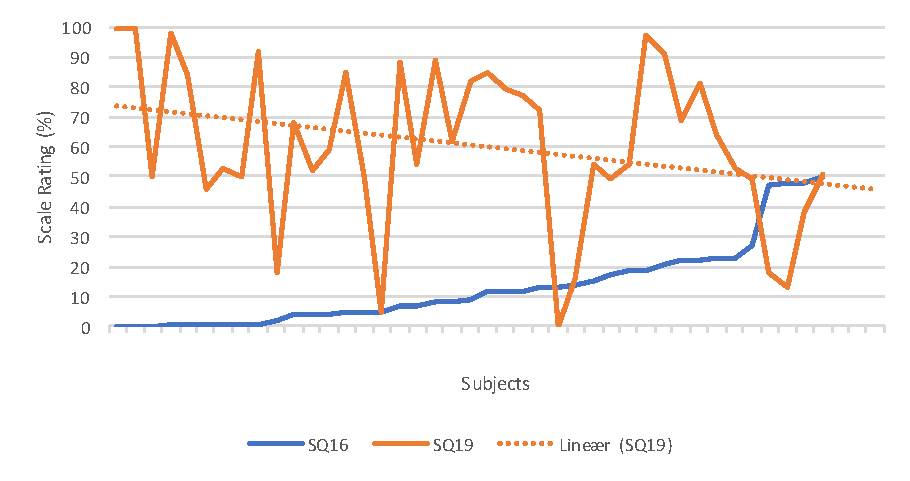
\includegraphics[width=\textwidth]{Figure/Korrelationsgrafer/SQ16+SQ19}
	\caption{Sammenhæng mellem hvad testpersonerne angiver (\%) på skalaen til SQ16 og SQ19, der begge har samme skala spørgsmål: \textit{Hvad synes du om robotten?}, men vedrører henholdvist \textit{irriterende} og \textit{sød}. Denne graf bygger på samtlige 43 besvarelser.}
	\label{fig:SammenligningSQ16SQ19}
\end{figure}
\noindent
%


\subsection{Korrelerede parametre fra afstand}
\label{DatabehandlingSammenligningKorreleredeAfstand}
%
Når PCA analysen udføres relativt til afstand, tyder det, som beskrevet i \fullref{DatabehandlingRAfstand}, på, at en positiv korrelation mellem følgende parametre forekommer:
%
\begin{itemize}
	\item SQ1 og SQ12
	\item SQ7 og SQ17
	\item SQ10 og SQ22
	\item SQ8 og SQ21\blankline
\end{itemize}
\noindent
%
Derudover forekommer der negativ korrelation mellem følgende parametre:
%
\begin{itemize}
	\item SQ2 og SQ9
	\item SQ5 og SQ8
	\item SQ5 og SQ21
	\item SQ10 og SQ13
	\item SQ13 og SQ22
	\item SQ14 og SQ16
	\item SQ19 og SQ20\blankline
\end{itemize}
\noindent
%
Sammenholdes SQ1 og SQ12 tyder det ikke på, at der er en korrelation mellem dem, hvorfor grafen forefindes i \fullref{ElektroniskBilagKorrelationsgrafer}. Selvom SQ17 kun har en minimal betydningen, fremgår det på \autoref{fig:Distance-Biplot}, at SQ17 er højt korreleret med SQ7, vedrørende robottens højde. Sammenholdes de to skala spørgsmål tyder det ikke på, at der er en korrelation mellem dem, hvorfor grafen forefindes i \fullref{ElektroniskBilagKorrelationsgrafer}.

Sammenholdes SQ10 og SQ22 tyder det ikke på, at der er en korrelation mellem hvor tryg testpersonerne er ved robotten og hvor sjov robotten opleves, jævnfør \autoref{fig:SammenligningSQ10SQ22}. 
%
\begin{figure}[H]
	\centering
	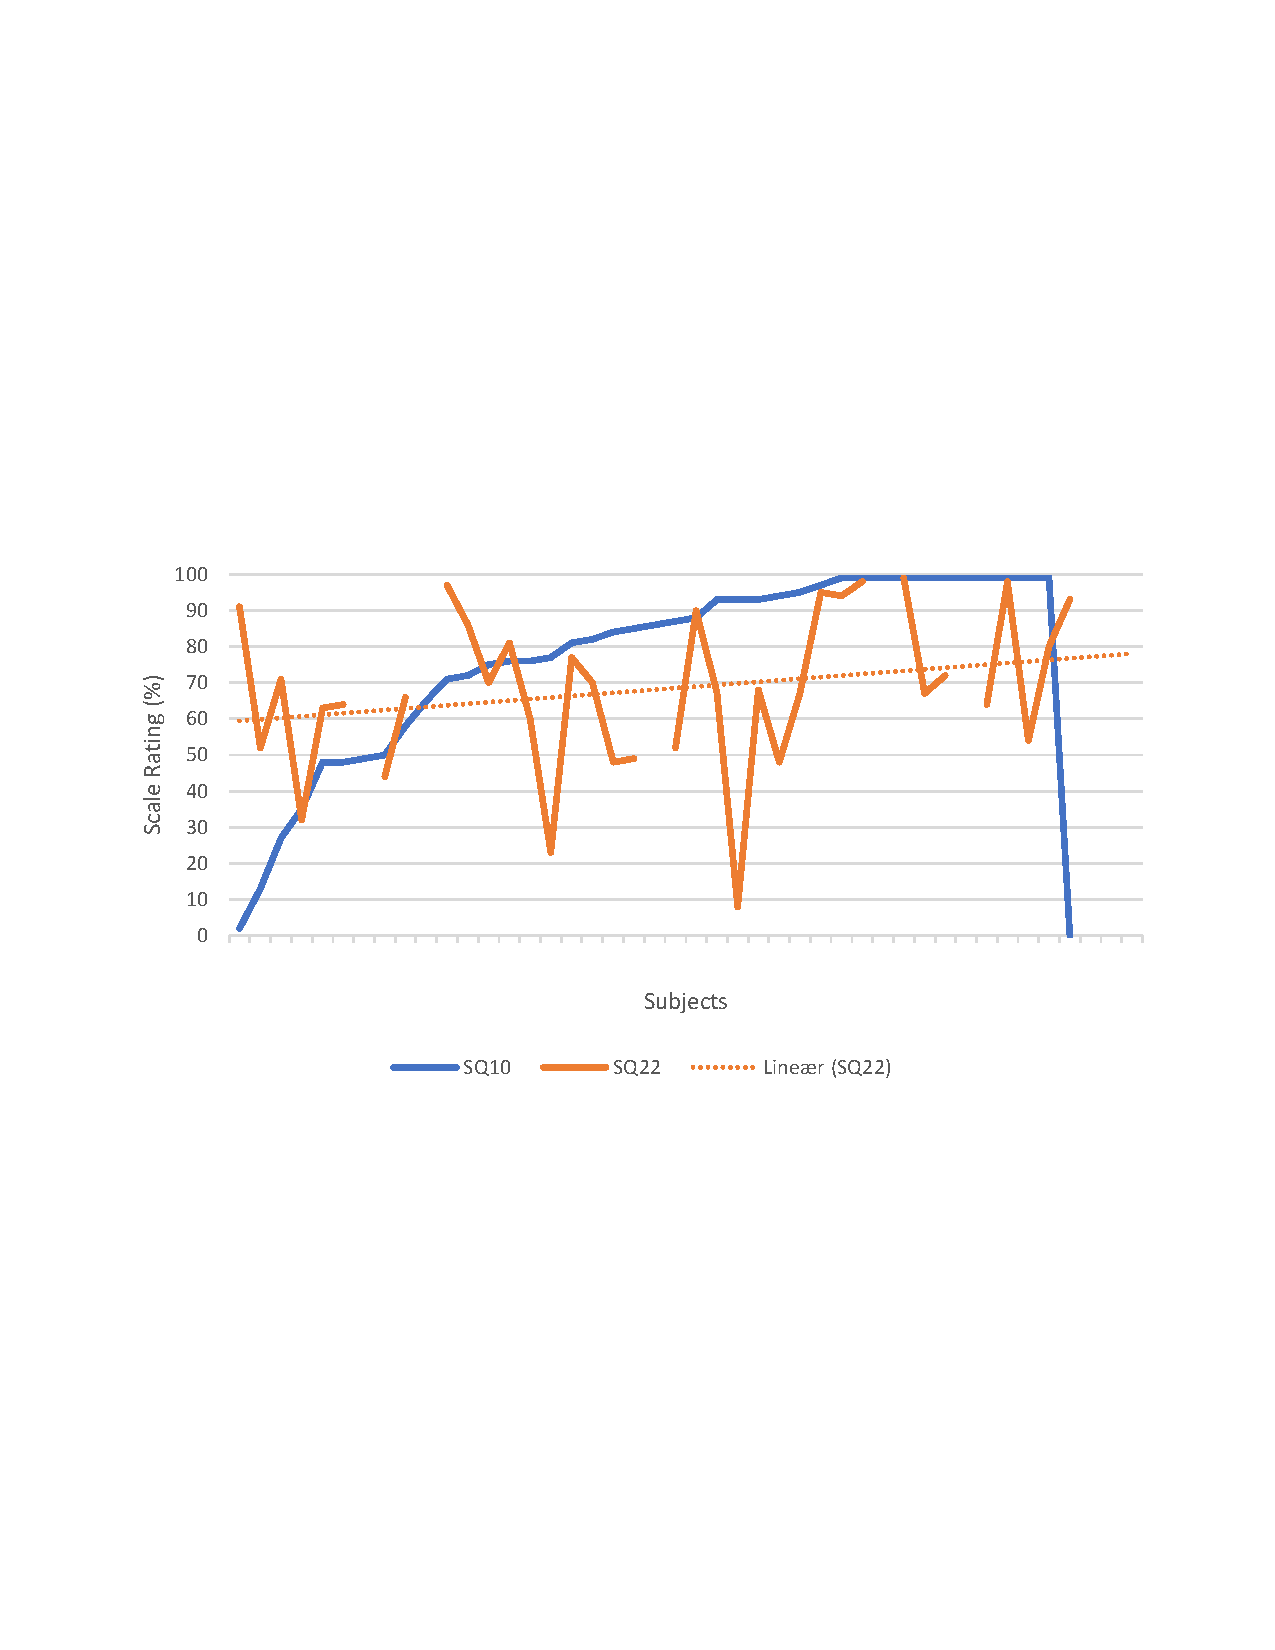
\includegraphics[width=\textwidth]{Figure/Korrelationsgrafer/SQ10+SQ22}
	\caption{Sammenhæng mellem hvad testpersonerne angiver (\%) på skalaen til SQ10: \textit{Jeg føler mig tryg ved robotten} og SQ22: \textit{Hvad synes du ellers om robotten?} i forhold til \textit{sjov}. Denne graf bygger på 35 besvarelser, da der manglede otte.}
	\label{fig:SammenligningSQ10SQ22}
\end{figure}
\noindent
%
Da der forefindes en positiv korrelation mellem SQ8 og SQ21 på \autoref{fig:Distance-Biplot}, forventes det, at tendenslinjen stiger, men når de to skala spørgsmål sammenholdes på \autoref{fig:SammenligningSQ8SQ21} tyder det ikke på, at det er tilfældet, jævnfør ingen korrelation.  
%
\begin{figure}[H]
	\centering
	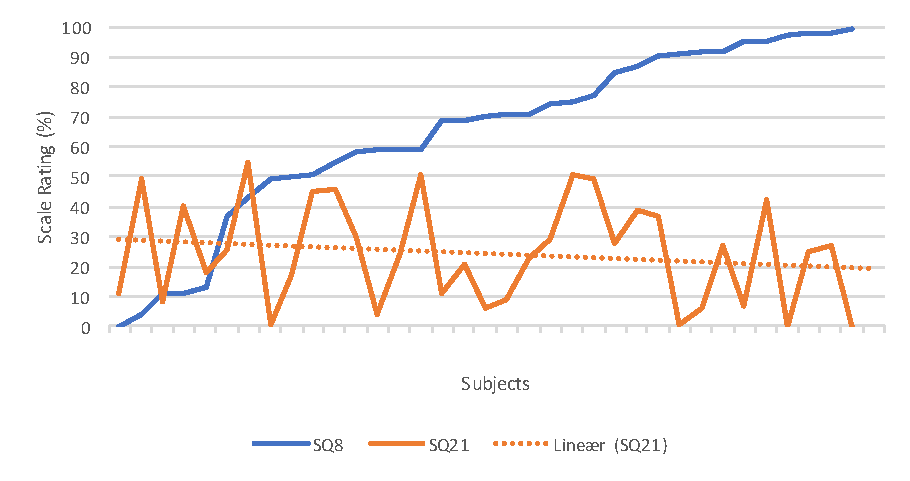
\includegraphics[width=\textwidth]{Figure/Korrelationsgrafer/SQ8+SQ21}
	\caption{Sammenhæng mellem hvad testpersonerne angiver (\%) på skalaen til SQ8: \textit{Jeg føler, at robotten kan hjælpe mig} og SQ21: \textit{Hvad synes du ellers om robotten?} i forhold til \textit{anmassende}. Denne graf bygger på 35 besvarelser, da der manglede otte.}
	\label{fig:SammenligningSQ8SQ21}
\end{figure}
\noindent
%
Den negative korrelation mellem SQ2 og SQ9 er præsenteret på \autoref{fig:SammenligningSQ2SQ9}. Sammenlignes SQ5 og SQ8, jævnfør \autoref{fig:SammenligningSQ5SQ8}, er det svært at udlede, hvorvidt der er en korrelation mellem de to parametre, da der forekommer stor variation i besvarelserne til SQ8. På trods af tidligere fundet negativ korrelation tyder det ikke på, at testpersonerne har en ændret oplevelse af om robotten kan hjælpe dem afhængigt af dens afstand. Det samme gør sig gældende, når SQ5 og SQ21 sammenlignes, hvorfor grafen forefindes i \fullref{ElektroniskBilagKorrelationsgrafer}. 
%
\begin{figure}[H]
	\centering
	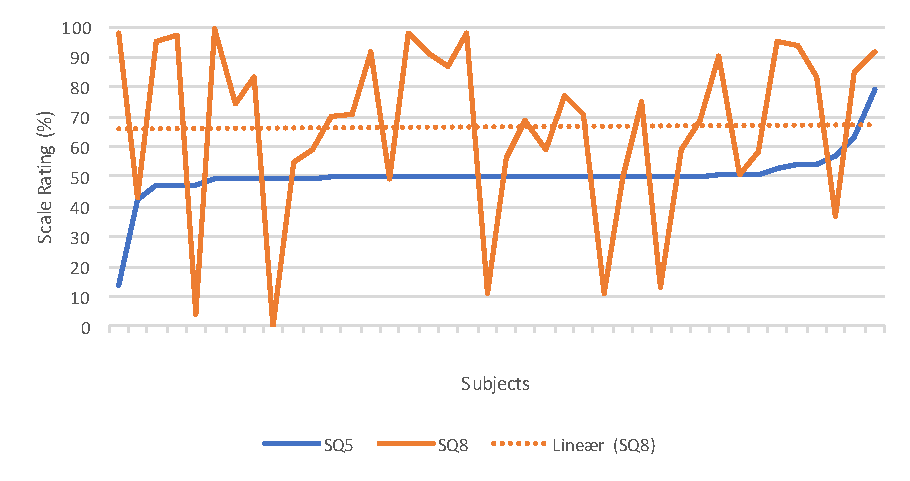
\includegraphics[width=\textwidth]{Figure/Korrelationsgrafer/SQ5+SQ8}
	\caption{Sammenhæng mellem hvad testpersonerne angiver (\%) på skalaen til SQ5: \textit{Jeg synes robotten stoppede...} og SQ8: \textit{Jeg føler, at robotten kan hjælpe mig}. Denne graf bygger på 40 besvarelser, da der manglede tre.}
	\label{fig:SammenligningSQ5SQ8}
\end{figure}
\noindent
%
Lignende er gældende for korrelationen mellem SQ13 og SQ22, hvor der heller ikke forefindes en negativ korrelation, men derimod tyder det på, at når testpersonerne regnede med at robotten fulgte dem hen til det valgte sted, så var de mere tilbøjelige til at vurdere robotten som værende mere sjov. Dog forekommer der en del manglende besvarelser til SQ22, hvorfor grafen for dette forefindes i \fullref{ElektroniskBilagKorrelationsgrafer}. 

Sammenholdes SQ14 med SQ16 tyder det ikke på, at der forekommer den før fundne negative korrelation, jævnfør \autoref{fig:SammenligningSQ14SQ16}.
%
\begin{figure}[H]
	\centering
	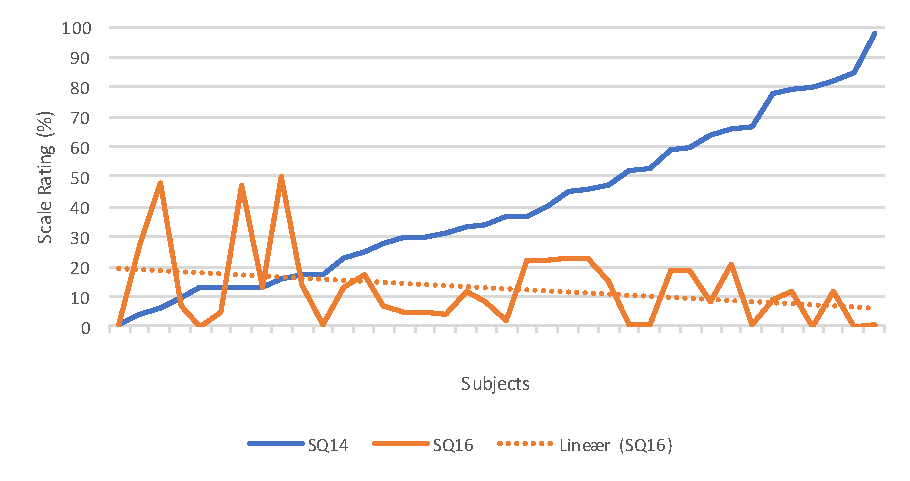
\includegraphics[width=\textwidth]{Figure/Korrelationsgrafer/SQ14+SQ16}
	\caption{Sammenhæng mellem hvad testpersonerne angiver (\%) på skalaen til SQ14: \textit{Hvor personlig oplevede du robottens hjælp?} og SQ16: \textit{Hvad synes du om robotten?}, i forhold til \textit{irriterende}. Denne graf bygger på 38 besvarelser, da der manglede fem.}
	\label{fig:SammenligningSQ14SQ16}
\end{figure}
\noindent
%
Sammenholdes SQ19 og SQ20 forefindes der ikke en negativ korrelation, men nærmere en postiv korrelation, jævnfør \autoref{fig:SammenligningSQ19SQ20}.
%
\begin{figure}[H]
	\centering
	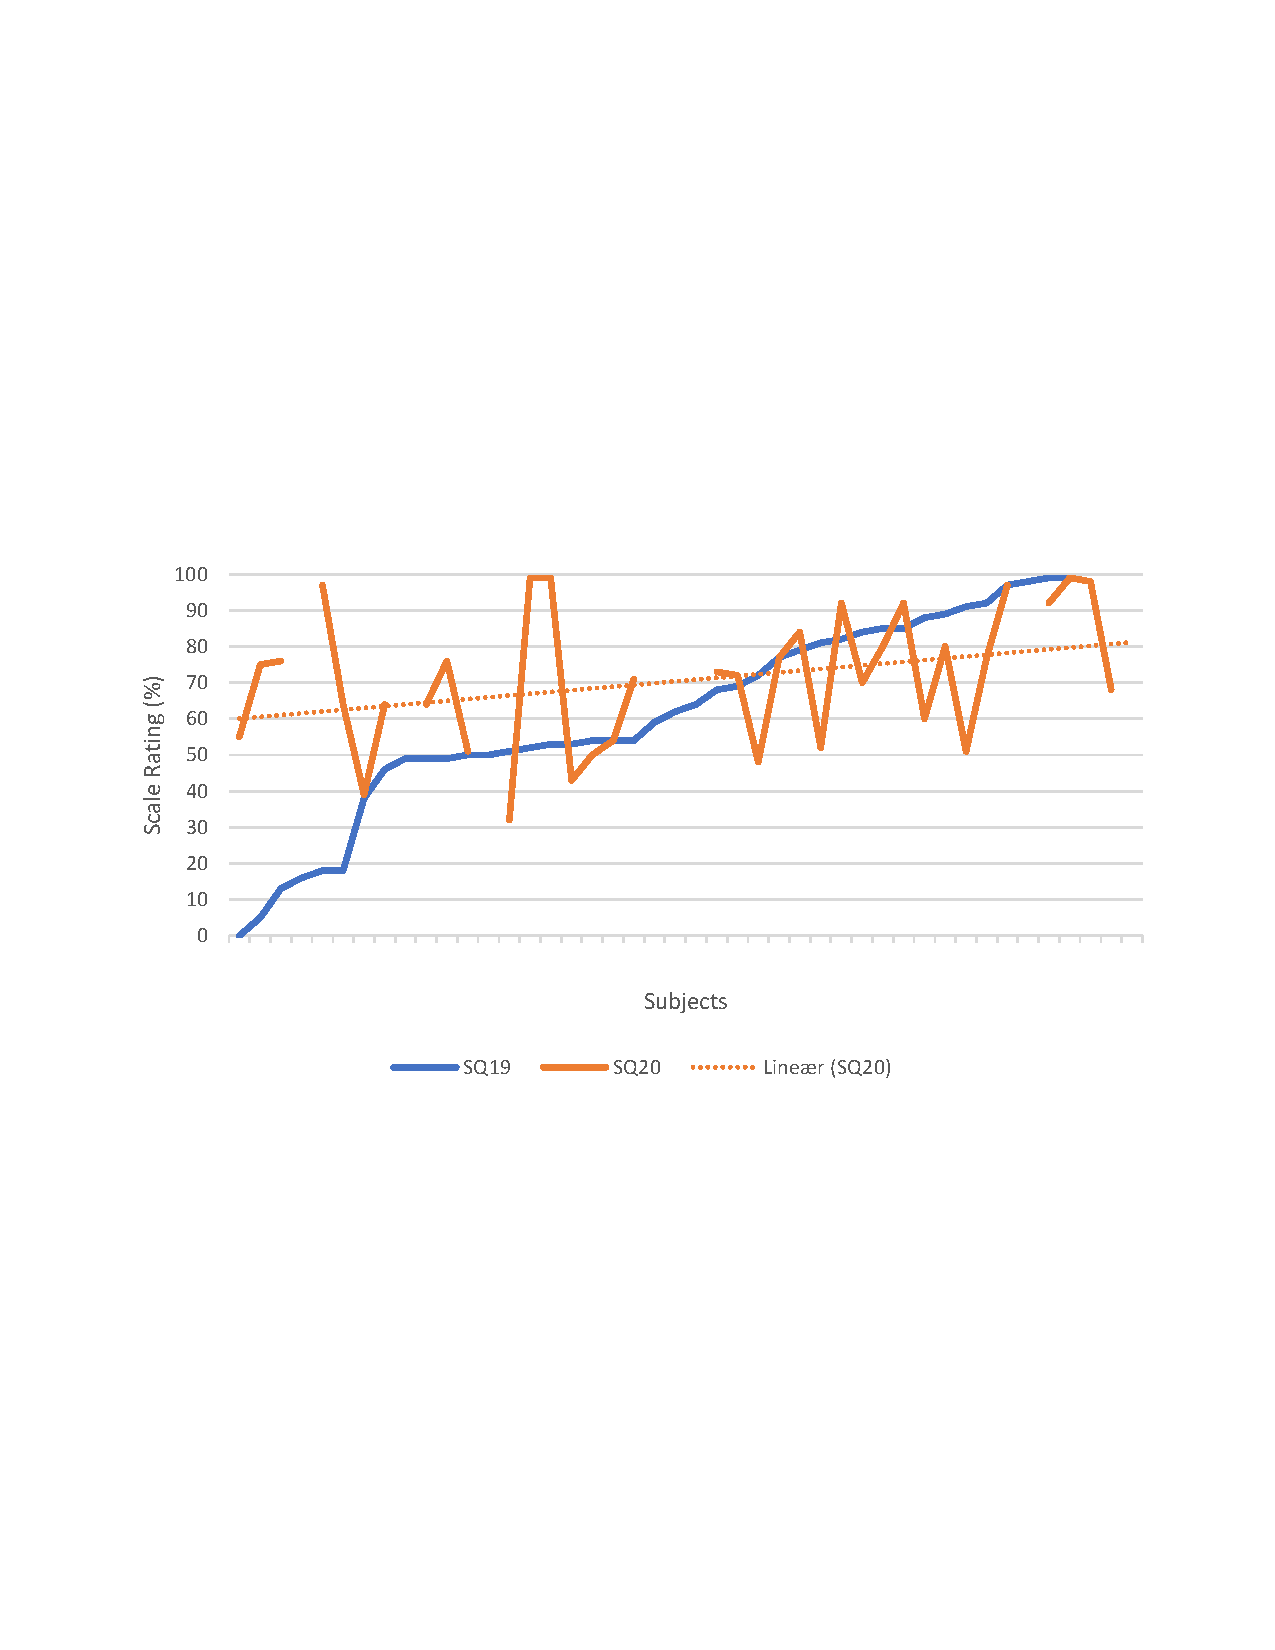
\includegraphics[width=\textwidth]{Figure/Korrelationsgrafer/SQ19+SQ20}
	\caption{Sammenhæng mellem hvad testpersonerne angiver (\%) på skalaen til SQ19: \textit{Hvad synes du om robotten?}, i forhold til \textit{sød} og SQ20: \textit{Hvad synes du ellers om robotten?}, i forhold til \textit{sej}. Denne graf bygger på 35 besvarelser, da der manglede otte.}
	\label{fig:SammenligningSQ19SQ20}
\end{figure}
\noindent
%



\subsection{Korrelerede parametre fra indgangsvinkel}
\label{DatabehandlingSammenligningKorreleredeIndgangsvinkel}
%
Når PCA analysen udføres relativt til indgangsvinkel, tyder det, som beskrevet i \fullref{DatabehandlingRIndgangsvinkel}, på, at en positiv korrelation mellem følgende parametre forekommer:
%
\begin{itemize}
	\item SQ8 og SQ10
	\item SQ9 og SQ14
	\item SQ5 og SQ7\blankline
\end{itemize}
\noindent
%
Derudover forekommer der negativ korrelation mellem følgende parametre:
%
\begin{itemize}
	\item SQ1 og SQ12
	\item SQ9 og SQ10
	\item SQ10 og SQ14
	\item SQ6 og SQ23
	\item SQ13 og SQ21\blankline
\end{itemize}
\noindent
%
Sammenholdes SQ8 med SQ10 tyder det på, at der er en positiv korrelation mellem de to skala spørgsmål, jævnfør \autoref{fig:SammenligningSQ8SQ10}. Dette medfører, at desto mere testpersonerne føler, at robotten kan hjælpe dem, desto tryggere er de ved robotten.
%
\begin{figure}[H]
	\centering
	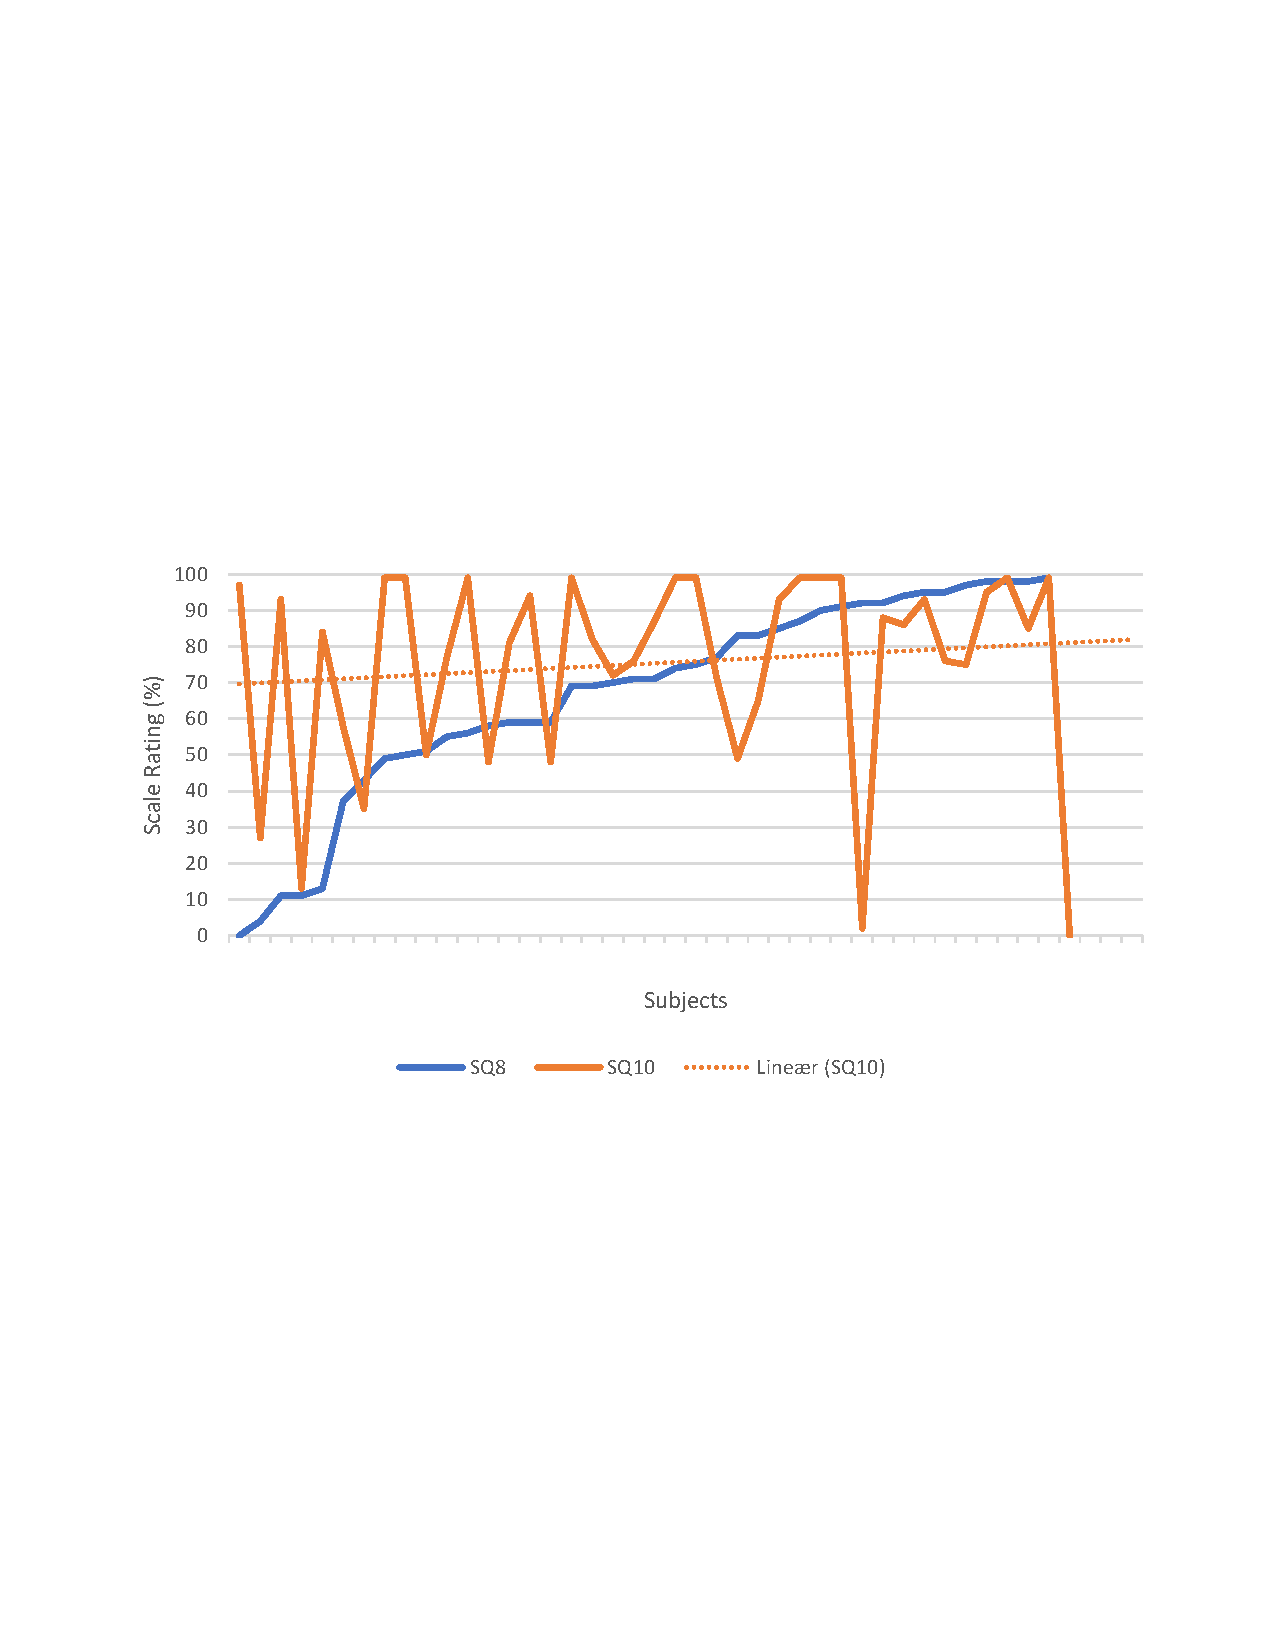
\includegraphics[width=\textwidth]{Figure/Korrelationsgrafer/SQ8+SQ10}
	\caption{Sammenhæng mellem hvad testpersonerne angiver (\%) på skalaen til SQ8: \textit{Jeg føler, at robotten kan hjælpe mig}, og SQ10: \textit{Jeg føler mig tryg ved robotten}. Denne graf bygger på 40 besvarelser, da der manglede tre.}
	\label{fig:SammenligningSQ8SQ10}
\end{figure}
\noindent
%
Selvom det ud fra \autoref{fig:Direction-Biplot} tyder på, at SQ9 og SQ14 er positivt korrelerede, så tyder det ikke på, at der er en korrelation mellem de to parametre, hvorfor grafen forefindes i \fullref{ElektroniskBilagKorrelationsgrafer}. Det samme gør sig gældende for SQ5 og SQ7, hvor det ikke tyder på, at der forekommer en korrelation, jævnfør \fullref{ElektroniskBilagKorrelationsgrafer}. For to af de negative korrelationer, tyder det ikke på, at der reelt er en korrelation. Dette gør sig gældende for SQ10 og SQ14 samt SQ6 og SQ23, jævnfør \fullref{ElektroniskBilagKorrelationsgrafer}.

Ud fra \autoref{fig:Direction-Biplot} fremgår det, at SQ1 og SQ12 er negativ korreleret, men når de to skala spørgsmål sammenholdes tyder det ikke på, at der overhovedet forekommer en korrelation, jævnfør \autoref{fig:SammenligningSQ1SQ12}.  
%
\begin{figure}[H]
	\centering
	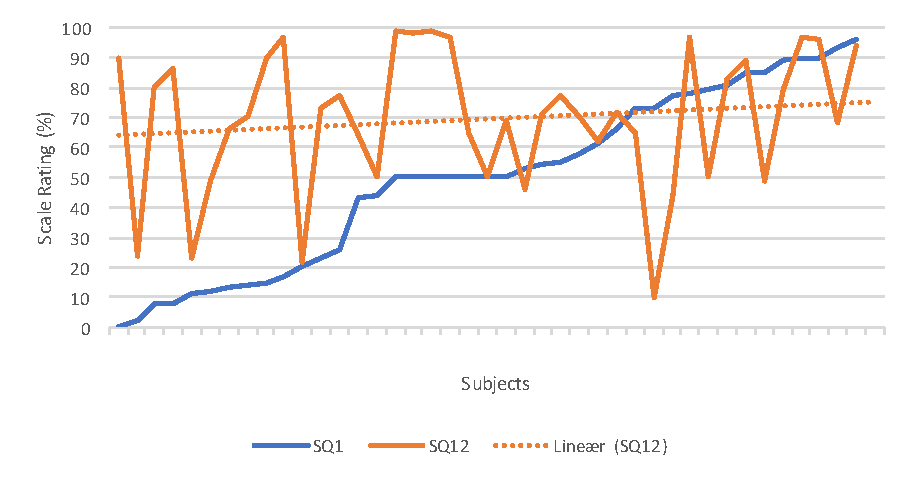
\includegraphics[width=\textwidth]{Figure/Korrelationsgrafer/SQ1+SQ12}
	\caption{Sammenhæng mellem hvad testpersonerne angiver (\%) på skalaen til SQ1: \textit{Hvordan synes du skærmen reagerede}, og SQ12: \textit{Jeg kan godt lide at blive betjent af robotten}. Denne graf bygger på 41 besvarelser, da der manglede to.}
	\label{fig:SammenligningSQ1SQ12}
\end{figure}
\noindent
%
Sammenlignes SQ9 og SQ10, jævnfør \autoref{fig:SammenligningSQ9SQ10}, forekommer der en lille korrelation relateret til at desto mere trygge testpersonerne er ved robotten, desto mindre synes de, at den stod i vejen. 
%
\begin{figure}[H]
	\centering
	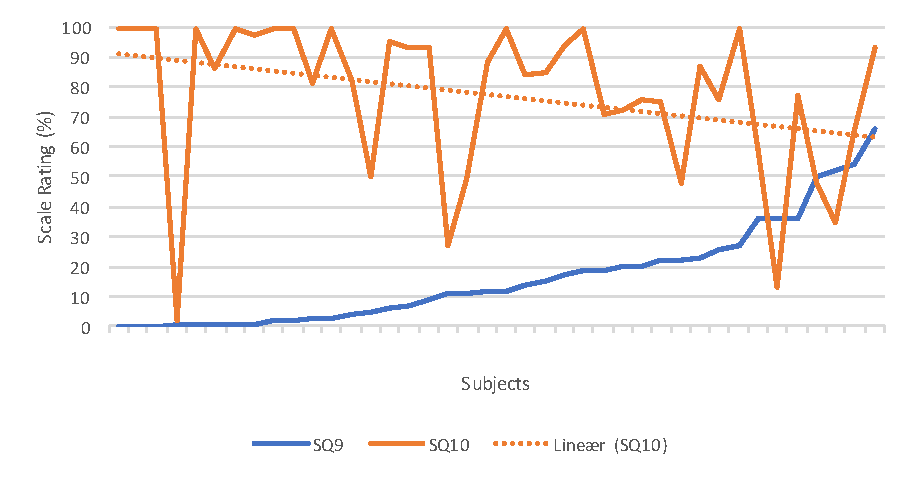
\includegraphics[width=\textwidth]{Figure/Korrelationsgrafer/SQ9+SQ10}
	\caption{Sammenhæng mellem hvad testpersonerne angiver (\%) på skalaen til SQ9: \textit{Jeg synes, at robotten stod i vejen} og SQ10: \textit{Jeg føler mig tryg ved robotten}. Denne graf bygger på 40 besvarelser, da der manglede tre.}
	\label{fig:SammenligningSQ9SQ10}
\end{figure}
\noindent
%
På \autopageref{fig:SammenligningSQ13SQ21} sammenlignes SQ13 og SQ21, hvor den negative korrelation vurderes til at være lille. Korrelationen vedrører at testpersonerne oplever robotten som værende mindre anmassende, desto mere de regner med at robotten følger dem hen til det valgte sted.
%
\begin{figure}[H]
	\centering
	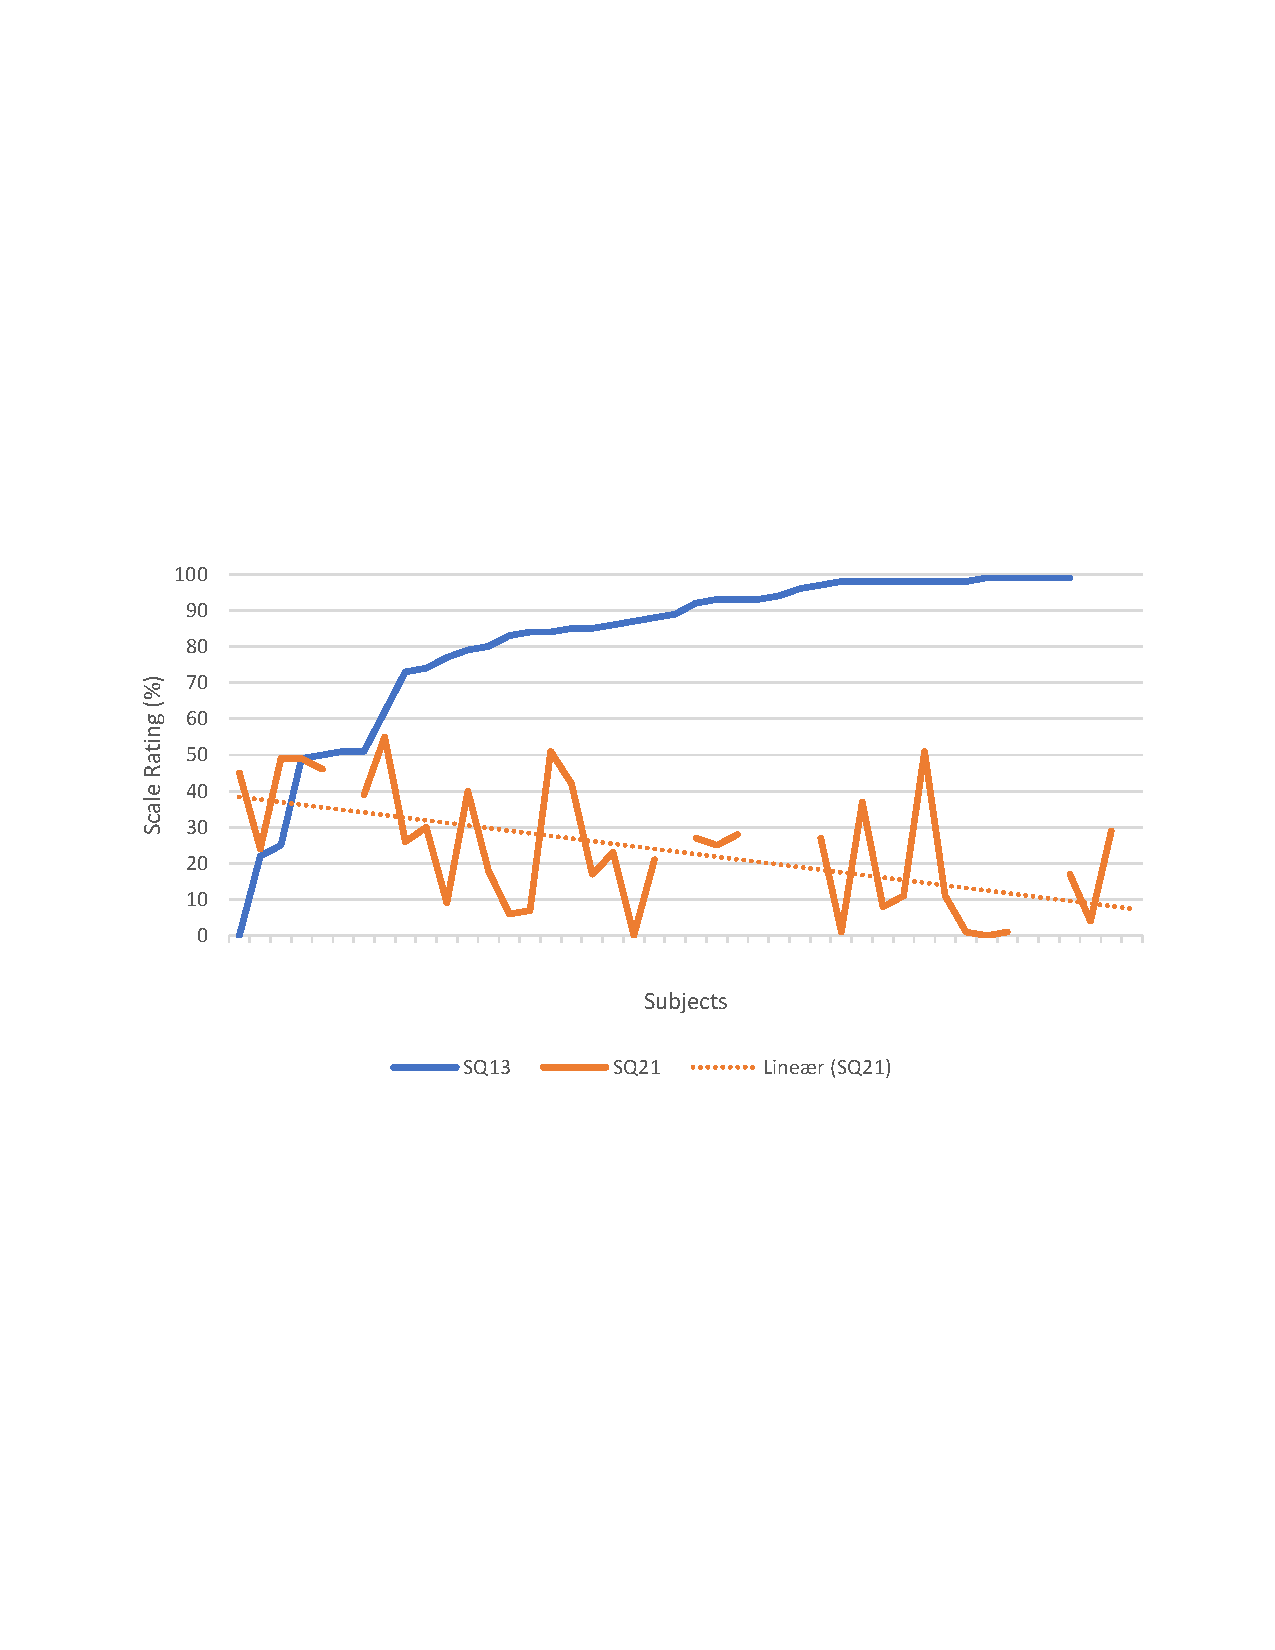
\includegraphics[width=\textwidth]{Figure/Korrelationsgrafer/SQ13+SQ21}
	\caption{Sammenhæng mellem hvad testpersonerne angiver (\%) på skalaen til SQ13: \textit{Jeg regnede med, at robotten fulgte mig hen til det sted jeg valgte} og SQ21: \textit{Hvad synes du ellers om robotten?}. Denne graf bygger på 35 besvarelser, da der manglede otte.}
	\label{fig:SammenligningSQ13SQ21}
\end{figure}
\noindent
%